\chapter{Progettazione e sviluppo}\label{chapter:formattazione}
In questo capitolo saranno esposti gli approcci teorici e pratici per lo sviluppo del progetto.

\section{Introduzione ai microservizi}\label{sec:cap_sec_subsec}
Prima di introdurre il concetto di architettura a microservizi è bene introdurre il concetto di architettura monolitica.\\
Un’architettura monolitica è una metodologia di sviluppo secondo la quale tutti i processi coinvolti sono strettamente legati tra di loro e sono erogati come un singolo servizio.\\
Questa tipologia di approccio porta ad avere sistemi nei quali modificare le funzionalità diventa più complesso in quanto si deve agire sull’intero sistema e non solo sulle parti effettivamente interessate.\\
Inoltre, utilizzare un’architettura monolitica porta a correre dei rischi per quanto riguarda la disponibilità dell’applicazione, in quanto anche se solo uno dei processi coinvolti avesse un malfunzionamento, questo si propagherebbe nell’intera applicazione.\\ \\
Per quanto riguarda le architetture a microservizi, queste sono diametralmente opposte alle architetture monolitiche.\\
Nelle architetture a microservizi l’obiettivo è quello di scomporre l’applicazione da realizzare nelle sue funzioni (\emph{servizi}) di base.\\
Ogni servizio può essere compilato e distribuito in modo indipendente; quindi i singoli servizi possono funzionare o non funzionare senza compromettere gli altri.\\
Utilizzare i microservizi significa riuscire a gestire criticità inevitabili, poter sfruttare la scalabilità dinamica e semplificare l'integrazione di nuove caratteristiche.\\ \\

\begin{figure}[ht]
	\centering
	\resizebox{1.0\textwidth}{!}{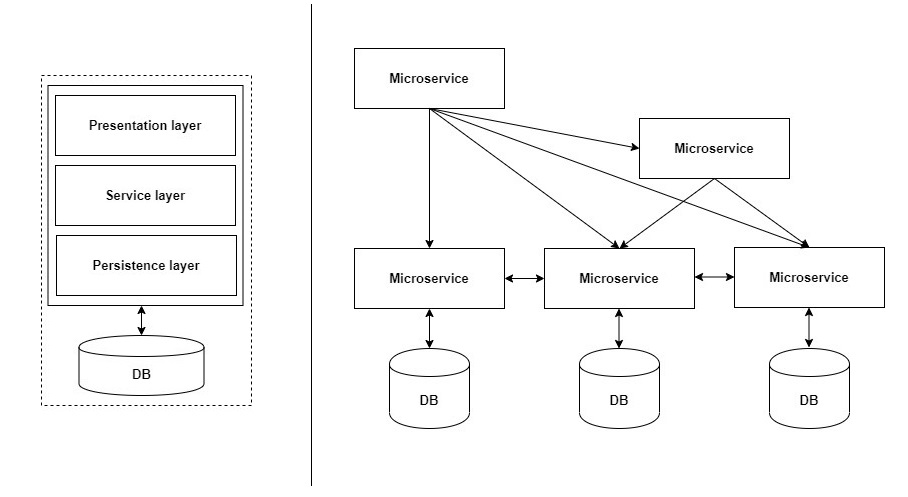
\includegraphics{img/monovsmicro}}
	\caption{Architettura monolitica e architettura a microservizi a confronto}
	\label{fig:one}
\end{figure}

Oggi i container Linux permettono di eseguire più parti di un'applicazione in modo indipendente con un controllo superiore sui singoli componenti.\\
I microservizi containerizzati rappresentano la base delle applicazioni cloud native.\\ \\
Di seguito sono elencati alcuni dei vantaggi di un’architettura a microservizi:

\begin{itemize}
	\item \textbf{Agilità}\\ Essendo ogni applicazione suddivisa in servizi di base, i team di sviluppo agiscono in contesti ridotti, semplificando il lavoro e ridurre i tempi del ciclo di sviluppo.
	\item \textbf{Scalabilità}\\Lavorare con un microservizio consente di scalare in modo indipendente per rispondere alla richiesta di un determinato servizio.\\ In questo modo è possibile misurare il carico di lavoro di un singolo servizio e adattarlo di conseguenza; il che può portare a dei vantaggi anche in termini economici per il mantenimento dell’applicazione. 
	\item \textbf{Semplicità di distribuzione}\\ I microservizi supportano l’approccio \emph{CI/CD} (Continuous integration/Continuous Delivery), così da semplificare l’integrazione e il testing di nuove funzionalità avendo comunque la possibilità di effettuare un rollback in caso di problemi.
	\item \textbf{Codice riutilizzabile}\\ Uno dei vantaggi del suddividere un’applicazione in servizi è la possibilità di poter riutilizzare codici di servizi già esistenti per altre applicazioni.
	\item \textbf{Resilienza}\\ Avendo un’applicazione a servizi indipendenti si aumenta la resilienza in caso di errori.\\ Si possono gestire completamente gli errori di un servizio isolando la funzionalità senza bloccare l’intera applicazione.

\end{itemize}



\section{Introduzione a Kong Gateway}\label{sec:cap_sec_subsec}
\section{Architettura del progetto}\label{sec:cap_sec_subsec}
\section{Architettura del microservizio}\label{sec:cap_sec_subsec}
\subsection{Sviluppo del microservizio}\label{sec:cap_sec_subsec}
\section{Architettura del plugin}\label{sec:cap_sec_subsec}
\subsection{Sviluppo del plugin}\label{sec:cap_sec_subsec}
